\section{Rozpoznanie twarzy}
Rozpoznanie twarzy zostało zrealizowane za pomocą otwartej biblioteki OpenCV opakowanej przez JavaCV w celu umożliwienia jej użycia przez język Java. Udostępnia ona szereg narzędzi ułatwiających rozpoznanie obrazu i jego dalszą obróbkę. Aby algorytmy poprawnie rozpoznawały twarze, został wygenerowany plik posiadający listę cech charakterystycznych dla twarzy. Generacja pliku polega na podaniu zestawu zdjęć "pozytywnych", czyli zawierających tylko twarze z frontu i profilu, zdjęć "negatywnych" ukazujących jedynie tła i środowisko w których twarze nie występują, oraz zwykłych zdjęć ludzi w zwykłym otoczeniu. 
Aby rozpoznać cechy typowe dla twarzy stosowane są algorytmy \textbf{Haara} i \textbf{Viola-Jones'a} (rozwiniętym przez Rainera Lienhart'a oraz Johena Maydt’a).

\subsection{Wybór zestawu cech}
W metodzie Viola-Jenes cechy traktowane są jako kombinacja dwóch, trzech lub czterech prostokątów. Ilość możliwych kombinacji połączenia prostokątów była bardzo duża, dlatego przy określonych założeniach została wyselekcjonowana grupa podstawowych cech. Następnie udoskonalony zestaw cech jeszcze lepiej identyfikujący poszukiwane obiekty został zaproponowany w metodzie Lienhart-Maydt. Grupa ta została podzielona na cechy krawędziowe, liniowe oraz centralnie otoczone. Właśnie z tego zestawu cech korzysta funkcja z OpenCV. Zasada działania cech polega na odnajdywaniu obszarów, na których różnica pomiędzy sumą pikseli regionów ograniczonych czarnymi i białymi prostokątami znajduję się powyżej pewnego progu. Na podstawie tej wartości algorytm może zidentyfikować czy badany obszar jest poszukiwanym obiektem czy jego tłem.

\begin{figure}[h]
\centering
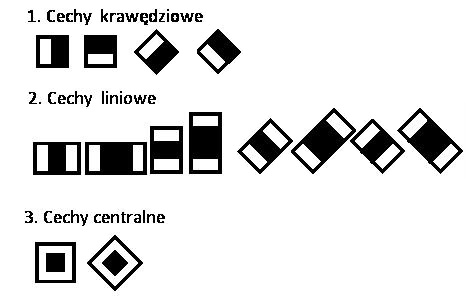
\includegraphics[scale=0.6]{./violajones.jpg}
\caption[Cechy rozpoznawane przez OpenCV]{Zestaw cech zaproponowany przez Lienhart'a i Maydt'a}
\end{figure}

Dla przykładu, prostokątne regiony oczu mają dużo mniejszą intensywnośd niż obszar czoła, ten zaś dużo większą od obszaru włosów 

\subsection{Tworzenie klasyfikatora kaskadowego}
Odbywa się z wykorzystaniem algorytmu uczącego \textbf{AdBoost}. Wykorzystuje on tzw. wzmocnienie adaptacyjne (ang. adaptive boosting). Jego
zadaniem jest wygenerowanie silnego klasyfikatoraz kaskady słabych. W przypadku obrazów, na których wykryty ma zostać obiekt wykorzystuje się technikę przesuwnego okna. Z tak zeskanowanego obrazu generowany jest zbiór okien, które poddawane są weryfikacji przez klasyfikatory. Na podstawie informacji z tych okien słabe klasyfikatory uczą się odrzucać obszary, na których na pewno nie znajduje się poszukiwany obiekt. W każdej pętli algorytm skupia się na źle wykrytych obszarach przez poprzednie klasyfikatory. Nadaje im wyższe wagi (gdyż w następnej iteracji istnieje większe prawdopodobieostwo prawidłowego wykrycia obiektu). Wykorzystywanie tych wag przez następne klasyfikatory pozwala na zawężenie przestrzeni poszukiwń do coraz mniejszego obszaru. Tak skonstruowany silny klasyfikator umożliwia szybkie wykrywanie poszukiwanych obiektów.
